\section{A Brief Review on Factorable Groups}
\label{notation:factorable_groups}

\begin{defi}
    \label{notation:height}
    \index{symmetric group!height of a permutation}
    \symbolindex[h]{$\height$}{The height of a permutation, i.e.\ the largest symbol which is permutated non-trivially.}{Definition \ref{notation:height}}
    Let $\alpha \in \Symgrp_p$ be a non-trivial permutation.
    The \textbf{height} of $\alpha$ is the largest symbol in the support of $\alpha$, i.e.\ 
    \[
        \height(\tau) = \max \supp(\alpha) \,.
    \]
\end{defi}

\begin{defi}
    \label{notation:factorization_map}
    \index{factorization map}
    \symbolindex[e]{$\eta$}{The factorization map which makes the symmetric groups factorable.}{Definition \ref{notation:factorization_map}}
    Let $G \subset \SymGr_p$ be the generating set consisting of all transpositions and the trivial permutation $1_{\SymGr_p}$.
    The {\bfseries factorization map} is
    \[
        \eta \colon \SymGr_p \to \SymGr_p \times G\,, \mspc{}{30} \alpha \mapsto (\ov\alpha, \alpha') 
    \]
    with
    \[
        \eta(1) = (1,1)
    \]
    and, for $\alpha \neq 1$,
    \[
        \ov\alpha = \alpha \alpha' \mspc{and}{35} \alpha' = (c\ \alpha^{-1}(c)) \mspc{for}{10} c = \hgt(\alpha) \,.
    \]
\end{defi}

\begin{rem}
    \label{notation:height_rem}
    For $\alpha \neq 1$, the height of $\alpha$ is permuted non-trivially by $\alpha'$ and a fixed point of $\ov\alpha$.
\end{rem}

% Kompiliert nicht ohne Klammern {\cite....}
\begin{thm*}[{\cite[Theorem 5.2.1]{Visy201011}}]
    The factorization map $\eta$ makes the symmetric group $\Symgrp_p$ factorable:
    Denoting the multiplication by $\mu \colon \SymGr_p \times \SymGr_p \to \SymGr_p$ in the diagram below,
    the upper right composition of maps preserves the norm if and only if the lower left composition does.
    In this case, the diagram commutes.
    \[
        \begin{tikzcd}
            \SymGr_p \times \SymGr_p  \arrow{d}{\mu} \arrow{r}{\eta \times \id} & \SymGr_p \times \SymGr_p \times \SymGr_p \arrow{r}{\id \times \mu}    & \SymGr_p \times \SymGr_p \arrow{r}{\id \times \eta}   & \SymGr_p \times \SymGr_p \times \SymGr_p \arrow{d}{\mu \times \id} \\
            \SymGr_p \arrow{rrr}{\eta}                                          &                                                                       &                                                       & \SymGr_p \times \SymGr_p
        \end{tikzcd}
    \]
\end{thm*}

It is handy to reformulate the above diagram as follows.
We start off with $2$ strings which represent the left respectively right factor of $\SymGr_p \times \SymGr_p$.
The composition of maps is now visualised by splitting a string into two parts if $\eta$ is applied, respectively by joining two strings if $\mu$ is applied.
We obtain the following Figure.
\[
    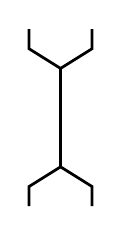
\begin{tikzpicture}[line width=1pt, yscale=.25, xscale=.8]
        \draw (1,9) -- (1,8) -- (.5,7) -- (.5,2) -- (1,1) -- (1,0);
        \draw (0,9) -- (0,8) -- (.5,7) -- (.5,2) -- (0,1) -- (0,0);
    \end{tikzpicture}
    \hspace{3cm}
    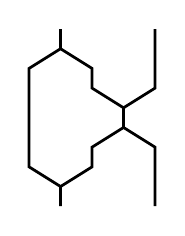
\begin{tikzpicture}[line width=1pt, yscale=.25, xscale=.8]
        \draw (0.5,9) -- (0.5,8) -- (0,7)                                         -- (0,2) -- (0.5,1) -- (0.5,0);
        \draw (0.5,9) -- (0.5,8) -- (1,7) -- (1,6) -- (1.5,5) -- (1.5,4) -- (1,3) -- (1,2) -- (0.5,1);
        \draw (2,9)   -- (2,6)                     -- (1.5,5) -- (1.5,4) -- (2,3)                     -- (2,0);
    \end{tikzpicture}
\]

